\documentclass[11pt, oneside]{article}

\usepackage[english]{babel}
\usepackage[utf8]{inputenc}
\usepackage{parskip} % for spaces between paragraphs
\usepackage[top=1.5in, bottom=1.5in, left=1.5in, right=1.5in]{geometry} % for custom margin sizes
\usepackage{amsmath}
\usepackage{amsthm}
\usepackage{graphicx}
\usepackage{algorithmicx}
\usepackage[colorinlistoftodos]{todonotes}
\usepackage{pslatex}
\usepackage[margin=1in]{geometry}
\usepackage{listings}
\usepackage{color}
\usepackage[margin=.25in]{caption}
\usepackage{subcaption}
\usepackage{tikz}
\usepackage{pgfplots}
\usepackage{verbatim}
\usetikzlibrary{automata,topaths}
\definecolor{mygreen}{rgb}{0,0.6,0}
\definecolor{mygray}{rgb}{0.5,0.5,0.5}
\definecolor{mymauve}{rgb}{0.58,0,0.82}
\newcommand{\ms}{\texttt}
\newtheorem*{lemma}{Lemma}

\lstset{ %
  backgroundcolor=\color{white},   % choose the background color
  basicstyle=\footnotesize,        % size of fonts used for the code
  breaklines=true,                 % automatic line breaking only at whitespace
  captionpos=b,                    % sets the caption-position to bottom
  commentstyle=\color{mygreen},    % comment style
  escapeinside={\%*}{*)},          % if you want to add LaTeX within your code
  keywordstyle=\color{blue},       % keyword style
  stringstyle=\color{mymauve},     % string literal style
}


\title{HODOR: HODOR On-Disk Orthogonal Range-trees}

\author{Stephanie Wang (swang93@mit.edu)\\
Bennett Cyphers (bcyphers@mit.edu)\\
Katie Siegel (ksiegel@mit.edu)\\[2ex]
6.851 Final Report}

\date{\today}

\begin{document}

\maketitle
\clearpage

\section{Introduction}

Many web applications today require data queries in two or more dimensions. For
instance, a point of interest on a map has latitude and longitude coordinates,
and may also be indexed by time, popularity, or other comparable values. A 
baseball player might be indexed by age, height, batting average, and salary;
movies in a streaming service could be sorted by year, user rating, length, etc. 
Databases typically support efficient range querying on one primary key at a
time. Multi-dimensional range queries, however, are expensive and require
several linear passes of the dataset in most implementations. 

As we have seen in class, orthogonal range trees are capable of range queries in
$d$ dimensions to $O(\log^{d-1} n + k)$ time, where $k$ is the size of the
result set [CITATION].  In-memory orthogonal range tree implementations have
been able to achieve significant query time speedup [CITATION, Tim's paper].
These can be used to extend a database for smaller datasets. Most datasets,
however, are too large to fit in memory, and therefore require an on-disk
implementation. To this end, we present HODOR, an on-disk Python implementation
of range-trees. 

The main obstacle in an on-disk implementation of orthogonal range trees is the
added overhead in disk access time. Therefore, in this paper, we explore
different methods of optimizing disk I/O accesses. First, we present
optimizations on the range tree structure itself. Second, we propose methods of
optimizing individual node serialization. Third, we explore optimizing the
serialization of the entire tree. Finally, we present results from benchmarking
these optimizations against a Python database [BUZHUG CITATION]. 

%%%%%%%%%%%%%%%%%%%%%%%%%%%%%% NEW BEGINNINGS %%%%%%%%%%%%%%%%%%%%%%%%%%%%%%%%%%aww

\section{Design}

\subsection{Goals}

The main goal of HODOR is to allow efficient range queries of very large
datasets with an arbitrary number of dimensions. We designed the structure to
perform on machines with a limited amount of memory and a large amount of
storage on a relatively slow hard disk. As such, we wanted to minimize the
time spent reading data from disk, but were generally unconcerned with
in-memory comparison operations. We optimized for this in two ways: first, by
minimizing total disk reads, and second, by chaining consecutive disk accesses
so that they can be executed as efficiently as possible. 

HODOR requires a relatively long time to construct its tree and serialize it to
disk, so the results presented in this paper are for queries on static trees
only. Although there are techniques, such as range trees with fractional cascading,
that can achieve a query speedup of a logarithmic factor, the goal here is more
to determine if we can achieve the same range query bounds on disk, rather than
to build the fastest structure possible.

\subsection{Range B-Trees}

The standard data structures used for implementing many table-style databases
are the B Tree, and its cousin, the B+ Tree. As a quick overview, a B tree is a
search tree with a branching factor of $B$; i.e., each node points to at most
$B$ children. The logic behind the B tree's design is that, since the act of
loading children from disk into memory is often the bottleneck on database
search performance, each node should load as many children as it can into memory
at once. $B$ can be tweaked to optimize for cache sizes on different machines.
A B-Plus tree is an extension of the B tree in which all data is stored at the
leaves of the tree, and each leaf has a pointer to its immediate predecessor
leaf, \ms{prev}. These predecessor pointers allow easy range queries in one
dimension by searching for the maximum value of the range and chaining together
predecessor leaves until the leaf containing the min value is reached.

The orthogonal range tree is a structure covered in 6.851 which allows $O(\log^d
n + k)$ range queries on $d$ dimensions, where $k$ is the number of data items
returned by the query. For HODOR, we extend the B-plus tree structure with
orthogonal, recursive linked trees to create a B-plus Orthogonal Range Trees
(BORT). Each node $n$ in a BORT has a dimension $d$, a set of $B$ child pointers
sorted in $d$, and a pointer to another BORT containing all of the data points
contained in $n$'s subtree, known as $n$'s \textit{linked tree}.  When $n$ is
loaded into memory, it brings with it all $B$ child pointers and one link
pointer.  Therefore, a search on $n$ data points indexed in $d$ dimensions
touches $O(log^d_B n)$ nodes, which requires $O(log^d_B n)$ disk accesses.
However, as we will describe below, not all disk accesses are equal, and we can
achieve better in-practice running times by laying out serialized nodes
intelligently on disk.

\subsection{Node serialization}

In order to store range trees on disk, we require an efficient method to
serialize and deserialize the data structure. In Hodor, we represent a Python
\texttt{RangeTree} instance as a list of serialized nodes, which may be
instances of \texttt{RangeNode} or \texttt{RangeLeaf}. This list is stored in a
``tree file", which can be written to and read by a \texttt{Serializer} class. 

During preprocessing, when building the tree from a set of datapoints,
\texttt{Serializer} is initialized in write mode to build the tree file.
\texttt{Serializer} in write mode exposes a \texttt{dumps(node)} method that
takes in a node instance, serializes the node, and appends it to the tree file.
This method also assigns the node a pointer into the tree file, which
is the number of nodes appended previously to it. 

Once the tree is fully built, we call \texttt{Serializer.flush()}, which
flushes the tree file to disk. From this point onwards, \texttt{Serializer} can
be used to read the tree.

In read mode, \texttt{Serializer.loads(pointer)} can be called to deserialize a
single node into a Python node instance, given its pointer into the tree file.
So, to give a parent access to its child, we simply store the child's tree file
pointer as an attribute of the parent. \texttt{loads} is implemented by seeking
the pointer in the tree file and reading out a single node's worth of bytes.

% maybe some of this should go into Implementation details maybe something
% about cPickle vs struct
The seeking method varies by serializer. In Hodor, we test two main node
serialization methods. The first is to use a delimiter, such as a newline
character, between nodes. The second is to pack nodes into fixed-length
strings, called ``blocks". 

\subsection{Tree serialization}


Tree serialization is executed while preprocessing the datapoints into a tree,
so that the order of nodes in the tree file is the same as the order in which
Hodor preprocesses them. The tree is built recursively, from the bottom up.
Hodor starts with a set of children. If these are leaves, then Hodor sorts them
by the current dimension. Next, Hodor partitions the children into clusters of
size $B$. For each of these clusters, Hodor creates a parent node and makes a
recursive call to build the parent's linked tree in the next dimension, if
there is one. If there is only one parent, then Hodor is done since the single
parent is the root.  Otherwise, Hodor uses the parents as the set of children
in the next recursive call. 

% TODO: fix formatting
\begin{figure}[p]
    \centering
    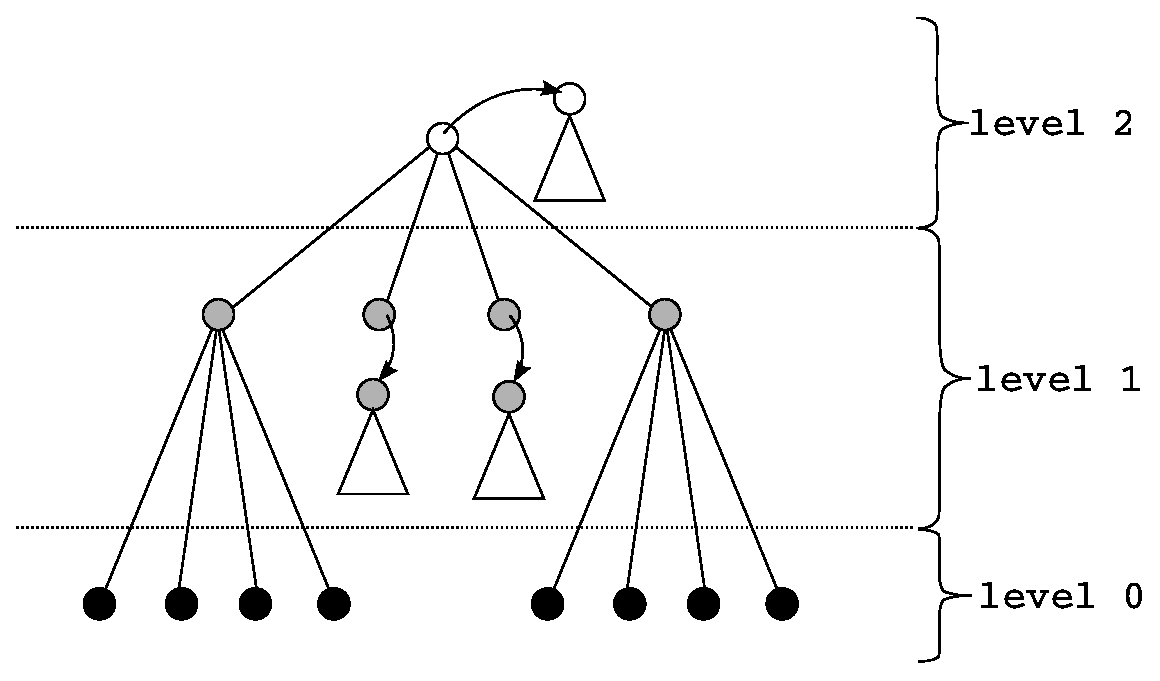
\includegraphics[width=0.8\textwidth]{fig1.eps}
    \caption{Awesome Image}
\end{figure}
\begin{figure}[p]
    \centering
    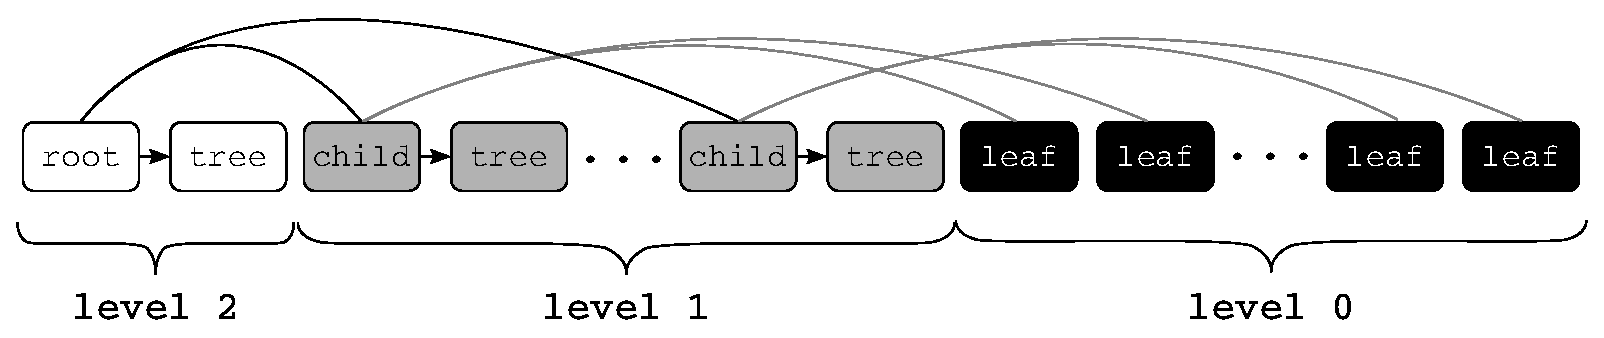
\includegraphics[width=1\textwidth]{fig2.eps}
    \caption{Awesome Image}
\end{figure}

% move fig 1 here
Hodor serializes the nodes in the same order that they are created. In the
recursion for a set of children, all children are serialized first, followed by
the linked subtree for each parent node, followed by the node itself. Each
child is serialized before its parent, and each parent is serialized
immediately after its linked subtree in the next dimension. This forms a series
of levels [FIGURE 1]. For any dimension, each node falls in the same level as
all of its siblings. The node's linked subtree in the next dimension also falls
in this same level. All of the node's children and their linked subtrees fall
in the level below, and the node's parent falls in the level above. 

All leaves of the tree in the first dimension are in that tree's lowest level,
and are therefore serialized first. The root of the same tree is in the tree's
highest level, and is therefore serialized last. The leaves and root of each
linked subtree follow the same pattern. 

% move fig 2 here
Once we finish building the tree, we flush the nodes in the tree file to disk
in reverse order of serialization. This way, each node will fall after all of
its ancestors [FIGURE 2]. In the final disk layout, the root of the tree in the
first dimension is the first node in the file, and the leaves of the same tree
are the last in the file. This layout allows us to always read forward through
the file as we traverse downwards from the root, as we do in a range query.
Since each node falls immediately before its linked subtree in the next
dimension, we also read forward through the file when traversing from one
dimension to the next. All of the siblings in one level were originally
serialized in order, so writing them to disk in reverse order means that within
each level, the maximum-valued sibling now comes first and the minimum-valued
now sibling comes last. 

\section{Analysis}

Our analysis assumes that HODOR is running on a machine with a high-capacity
spinning disk for long-term storage, and a smaller main memory with fast 
reads and writes.

In our analysis, we will focus on measuring disk reads in two categories.
Assuming we are reading blocks from one continuous file on disk, \textit{forward
seeks} are defined as reads from a location after the current file pointer, so
that the pointer's value is increased. \textit{Back seeks} are reads from a
location before the current pointer, so that the pointer's value must be
decreased. In our disk-memory model, forward seeks are, in general, much faster
than back seeks. When accessing file blocks in sequential order, the blocks can
be loaded into memory at speeds approaching the disk's maximum read speed, which
is on the order of 100MB/s on modern hard drives. However, if a file block from
position $i-1$ is accessed immediately after the file block at $i$, the disk
must make most of complete revolution before the new block can be loaded. On a
typical drive spinning at 7200 RPM, this revolution takes over 8 milliseconds.

% make a note of mixing front and back seeks --> more jumps

In addition to minimizing total disk reads, we tried to minimize back seeks
wherever possible when designing HODOR. We will analyze our data structures in
terms of both total reads and total back seeks in the sections below.

\subsection{BORTs}

We will now examine the complexity of a search on a fully formed BORT, in terms
of total disk reads. The algorithm for performing a range query on a (non-leaf)
node is as follows, in pseudocode. Here, \ms{ranges} is a dictionary of the
ranges to be sorted, indexed by the name of each range's dimension. The BORT has
$n$ total elements, $d$ dimensions, and a branching factor of $B$.

\begin{algorithm}
    \caption{Finding all nodes in ranges in multiple dimensions}
    \begin{algorithmic}[1]
        \Require{\nod\textsc{Ranges} is a dictionary of (start, end) tuples indexed by
        dimension, and $d$ is the dimension of the current node.}
        \Statex
        \Function{RangeQuery}{\textsc{Ranges}, $d$}
            \Let{$start, end$}{Ranges[$d$]}
            \If{$z_i \neq 0$}
            \Let{$\delta$}{$\delta + 1$}
            \EndIf
          \EndFor
          \State \Return{$\delta$}
        \EndFunction
    \end{algorithmic}
\end{algorithm}
\textsc{RangeQuery}(ranges, dimension): \\
    start, end $<-$ ranges[dimension] \\
    
    if IS\_LAST\_DIMENSION: \\
        return \textsc{GetRange}(start, end) \\

    \textsc{GetResultsFor}(children\_in\_range(start, end)) \\

    Recurse on child containing start \\
    Recurse on child containing end

In the base case, the node is in the last dimension, and the function is reduced
to a \ms{get\_range} call. \ms{get\_range} is a function which returns all
leaves in the range in this node's subtree. It is accomplished by searching for
the leaf containing \ms{end}, and walking backwards along the link's \ms{prev}
pointers until the leaf containing the minimum value is found. This operation
takes $O(\log_B n + \frac{k}{B})$ reads, since each leaf contains $B$ elements.

Otherwise, the algorithm makes three recursive calls. First, the node finds all
$O(B)$ of its children which are fully contained within the range on its
dimension. It recurses on the \ms{linked\_node} for each one, essentially
initiating a new range query on $O(\frac{n}{B})$ elements and $d - 1$
dimensions. Next, it recurses with the same query on the two child nodes
containing \ms{start} and \ms{end}, each of which is a BORT with $\frac{n}{B}$
elements total.

Not shown is the logic at the leaf level. However, once \ms{range\_query} is
called on a leaf, the leaf can either return some subset of its data (requiring
no more disk reads) or recurse on a linked leaf in the next dimension (requiring
exactly one disk read per dimension, for $O(d)$ disk reads total).

In total, each higher-level recursive call involves $O(B)$ disk reads, and
recurses on $(O(\frac{n}{B})$ elements in its own dimension and $O(n)$ elements
in the next dimension; the base case involves a maximum of $O(\log_B n +
\frac{k}{B})$ reads. Therefore, running the entire algorithm from the root node
of a BORT makes $O(\log_B^d n + k)$ reads from the disk. In the sections below,
we will analyze how we can bound the \textit{types} of disk reads we have to
make.

\subsection{Node serialization}

In Hodor, we test two methods of node serialization: one with varible-length 
delimited strings, and one with fixed-length blocks. Both of these methods see a
trade-off between convenience and efficiency. 

Delimited strings are convenient because they support arbitrarily sized
datapoint values. In addition, the delimited method may help to keep down the
range tree's space overhead, since nodes are packed tightly. However, seeks may
be costly in performance, since a node's exact byte position in the file cannot
be calculated without reading from the file and counting delimiter characters.
This may be mitigated by Python's line iterator or linecache features
[CITATION, f.lines() iterator, linecache]. 

Loading nodes from fixed-length blocks yields a lower performance cost than
from delimited strings. When nodes are stored as blocks, a node's exact byte
position can be calculated from its file pointer, so Hodor can jump to nodes
directly. However, fixed-length blocks are less flexible in space usage than
delimited strings. Each node in a range tree stores a constant number of
values, such as min, max, and child pointers, and each leaf stores the values
for $B$ data points. If we bound the size of each node and leaf, we can
serialize each node with efficient space usage. However, this limits the type
and size of data that can be stored. Data points with variable-length data types
like strings

To support arbitrarily sized data in constant sized blocks, we can store the
data points themselves as delimited strings at the end of the database file, and
store pointers to the data in the leaves. When a query is performed, the
pointers can all be read into memory first, sorted, and used to access the
actual data sequentially from the file. This method requires $k$ extra disk
reads, but no extra back seeks.

% stats on block serializer vs line serializer here?

\subsection{Tree serialization}

% analyze a range query in terms of back seeks

The efficiency of tree serialization in terms of back seeks depends on the path
taken by a range query. We want to order the node accesses during a range query
so that we do as many consecutive forward seeks as possible, while minimizing
back seeks. Here we review a typical implementation of the range query
recursion and analyze its worst-case back seek count. 

% treat base case of the recursion separately

A range query algorithm starts from the root of the tree in the first dimension
and works recursively as it traverses down each tree and through the
dimensions, treating each node as the root of its subtree. For each of the
root's children, the range query either makes a recursive call on the child's
linked subtree, the child itself, or not at all. If the child's range lies
completely within the queried interval, the algorithm recurses on the child's
linked node, the root of the child's linked subtree in the next dimension. If
this isn't the case, and if the child's range contains the start- or end-point
of the queried interval, the algorithm recurses on the child itself. Otherwise,
the algorithm makes no other recursive call. 

As discussed above, the nodes are structured into recursive levels on disk,
where each level contains a node, all of its siblings, and its linked subtree
in the next dimension. The number of back seeks we do during each recursion
depends on the order in which nodes of the same level are accessed and the
order in which the levels themselves are accessed. Each level is sorted in
reverse order, so if a node is accessed after its left sibling, it will cost
one back seek. For each tree, the levels themselves are sorted in order from
highest to lowest, so if an ancestor is accessed after the node itself, it will
also cost one back seek. 

Because a node and all of its siblings lie in the same level, when the range
query accesses the root's children, all work is done in the same level.  Each
level is sorted in reverse order in the file, so if the range query accesses the
children from max to min (right to left), then no back seeks are needed to load
the root's children. Finally, the algorithm recurses on several child nodes, for
which all of the data is located later in the file. Because the range query
always traverses downwards in the tree, we never return to the root's level once
we access the children's level.

Next we analyze the back seeks needed for a recursive call on a child node.
There are two possible types of recursive calls: either we recurse on the
node's linked subtree, or we recurse on the child node itself. 

In the first case, note that the entirety of each node's linked subtree falls in
the same level as the node, and the subtree occurs immediately after the node in
the disk layout. Therefore, the recursive call on the subtree stays within the
same level as the node, and the file pointer only seeks forward. Additionally,
since the linked subtree immediately follows its node, we can make each
recursive call to a linked subtree directly after loading the child to avoid
back seeks within the same level. Thus, a recursion in the first case does not
require any back seeks.

In the second case, the range query recurses on the current node, in the same
way described above, and loads the node's children. According to the level
structure of the tree file, the current node's children all lie in the next
level, which can be reached by seeking forwards. However, if the range query
ever has to access the current node's level again, a back seek will be needed to
return from the children's level, or from even further down the tree.  This
happens whenever a second-case recursive call on a node is followed by a
recursive call on one of the node's siblings: the file pointer will follow the
first node's subtree to a lower level, and will have to jump back up to the
sibling's level for the second recursion. In other words, for the current root,
all recursive calls of the second case will count for one back seek, except for
the very last call made. 

\begin{lemma}
    According to the given algorithm, there will be at most $O(\log_B^dn)$ many
    back seeks.
\end{lemma}
\begin{proof}
\end{proof}

The given range query algorithm requires back seeks because of the accesses to
a level that we have already previously traversed past. If we can eliminate
these accesses from the naive algorithm, it will be possible to get no back
seeks at all. To achieve this, we need to ensure that by the time we traverse
downward from some node, all work that will ever be done in that node's level
has already finished. The work done on that node's level is the work involving
that node, its children, and its linked subtree in the next dimension. Here, we
propose a modified algorithm that accomplishes this and analyze its complexity
in back seeks.

Like the naive algorithm, the modified algorithm starts at the root of the tree
in the first dimension. However, rather than recursing on one node at a time,
the modified algorithm recurses on a set of nodes, or more accurately a set of
siblings. Similar to before, the algorithm determines which out of the current
set of nodes cover ranges that fall completely within the queried interval. For
these nodes, the algorithm makes a recursive call to the linked nodes, as in
the naive algorithm. However, for the second case of the recursive call, when a
node in the current set has a range containing the start- or end-point of the
queried interval, the algorithm does not recurse immediately on that node's
children. Instead, the algorithm collects the children of all such nodes in the
current set, and recurses on the union of the children.

% prove that the current set of nodes is all in the same level, so that we can
% guarantee no back seeks between nodes in the current set
To show that the modified algorithm does not require any back seeks, we first
prove that for any recursive call, the nodes in the current set are all
siblings. If this is true, then all the nodes in the current set will fall
within the same level. Then, if we do our work for each sibling in reverse
order, the order in which the siblings are laid out on disk, we will avoid any
back seeks between nodes in the current set.

\begin{lemma}
    For any recursive call during the modified algorithm, the set of nodes that
    is recursed upon is a set of all siblings.
\end{lemma}
\begin{proof}
    We can prove this by showing that it is an invariant. Assume that the nodes
    in the set for the current recursion are all siblings. From here, we may
    recurse on the root of a node's linked subtree or we may recurse on the
    combined children of some number of nodes in the current set. In either
    case, any recursive call that we make will be on a set of nodes that are
    all siblings. We begin the entire range query from a set of one, the root
    of the tree in the first dimension. Therefore, any recursive call that we
    make will be upon a set of nodes that are all siblings. 
\end{proof}

% prove that we never need to come back to this level
Since we do not require any back seeks between nodes in the current set, the
only other possible source of back seeks is from the recursive calls. We know
from the lemma that the current set of nodes for a recursion is in the same
level. The case when we do a recursive call on one of the nodes' linked
subtrees is then the same as in the naive algorithm; these do not cost any back
seeks since we remain in the same level and can do all the recursive calls in
order of disk layout. 

The other case is when we do a recursive call on the union of some nodes'
children. In this case, we are accessing the level after the current set's
level. If we do this recursive call after recursing on the linked subtrees, we
will never need to return to the current nodes' level, and will therefore not
need any back seeks following this recursive call. Thus, each recursion, and
therefore the modified algorithm as a whole, does not require any back seeks.

\subsection{Results}

% stats
\begin{figure}[b!]
\centering
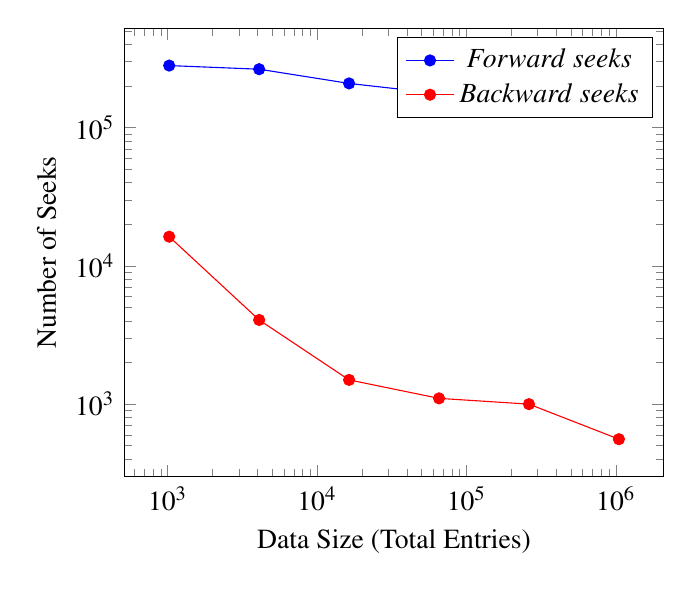
\begin{tikzpicture}
	\begin{loglogaxis}[
		xlabel=Data Size (Total Entries),ylabel=Number of Seeks]

	\addplot[color=blue,mark=*] coordinates {
		(1024,280524)
		(4096,264056)
		(16384,208401)
		(65536,176031)
		(262144,164698)
        (1048576,156474)
	};
	\addplot[color=red,mark=*] coordinates {
		(1024,16250)
		(4096,4061)
		(16384,1497)
		(65536,1101)
		(262144,1000)
        (1048576,558)
	};
	\legend{$Forward\ seeks$,$Backward\ seeks$}
	\end{loglogaxis}%
\end{tikzpicture}%
\caption{
    The number of forwards and backwards seeks invoked by range queries varies
    with the size of the data set in the orthogonal range tree. While
    backwards seeks are far more costly than forward seeks, they are far
    fewer in number, and the number of back seeks as a fraction of total seeks
    decreases exponentially as the set of data points grows.
}
\label{fig:figure2}
\end{figure}

\section{Conclusion}

% note about our model: we've dealt with things in terms of time and space
% before, and we dealt with disk accesses in cache-obliviousness, but this is
% cool ... and stuff

\section{References}

\noindent

\begin{description}

\item item

\end{description}
\end{document}
